\documentclass[twocolumn]{article}

\usepackage[utf8]{inputenc}
\usepackage[margin=0.85in]{geometry}
\usepackage{authblk}
\usepackage{setspace}
\usepackage{graphicx}
\graphicspath{{./figures/}}
\usepackage{subcaption}
\usepackage{amsmath}
\usepackage{booktabs}
\usepackage{hyperref}
\usepackage{tabularx}
\usepackage{enumitem}
\setlist{nosep,leftmargin=*}

\setlength{\columnsep}{20pt}

%%%%%% Bibliography %%%%%%
\usepackage[
  style=nejm,
  citestyle=numeric-comp,
  sorting=none
]{biblatex}
\addbibresource{sample.bib}

%%%%%% Title %%%%%%
\title{Sub-Terrain Challenge: Autonomous Cave Exploration with a Quadrotor UAV\\
\large Group 16 -- Autonomous Systems WS25/26}

%%%%%% Authors %%%%%%
\author[1]{Yujia Wang}
\author[1]{Ziming Liu}
\author[1]{Jiacheng Li}
\author[1]{Nihat Ak{\i}n}
\author[1]{Iliasu Olayiwola Salaudeen}

\affil[1]{Technical University of Munich, Munich, Germany.}

\date{March 3, 2026}

\setstretch{1.1}

\begin{document}
\twocolumn[
\begin{@twocolumnfalse}

\maketitle

\begin{abstract}
We describe the design and implementation of our autonomous quadrotor system for the Sub-Terrain Challenge.
The drone is tasked with exploring a simulated cave, building a 3D voxel map, and locating four lantern objects as fast as possible.
Our pipeline runs on ROS\,2 Jazzy and connects to an instructor-provided Unity simulation through a TCP/UDP bridge.
Depth images are converted to point clouds and fused into an OctoMap occupancy grid.
An A* planner generates collision-free paths, which are smoothed into time-parameterized trajectories with a trapezoidal velocity profile.
An SE(3) geometric controller, also provided with the course material, tracks the trajectory and sends rotor commands back to the simulator.
Lantern detection is achieved through semantic segmentation fused with depth data.
\end{abstract}

\vspace{0.8em}
\end{@twocolumnfalse}
]

%%%%%%%%%%%%%%%%%%%%%%%%%%%%%%%%%%%%%%%%%%%%%%%%%%%%%%%%%%%%
\section{Introduction}

The Sub-Terrain Challenge requires an autonomous UAV to enter a cave environment, find four lantern objects, report their positions, and produce a 3D representation of the explored space.
The entire system runs inside a Unity-based simulation, interfaced through ROS\,2.
The course provided several base packages---the Unity simulation bridge, a geometric SE(3) flight controller, and MAV message definitions---on top of which we built our own perception, detection, planning, mapping, and mission-management modules.
In total the workspace contains 14 ROS\,2 packages.
Our main design goal was to keep our own packages independent so that team members could develop and test in parallel.
This report gives an overview of the architecture, describes the algorithms we implemented, and documents who contributed what.

%%%%%%%%%%%%%%%%%%%%%%%%%%%%%%%%%%%%%%%%%%%%%%%%%%%%%%%%%%%%
\section{System Architecture}

The system begins at the simulation bridge, which receives raw sensor data from Unity via TCP and publishes it as standard ROS\,2 messages.
Perception nodes convert depth images into 3D point clouds and then into an OctoMap occupancy grid.
A separate detection node finds lanterns by fusing the semantic camera with depth.
The path planner reads the occupancy grid and the current goal, runs A* search, and outputs a waypoint path.
The trajectory planner turns this path into a smooth, time-parameterized trajectory.
Finally, the SE(3) controller computes rotor speed commands, which are sent back to Unity over UDP.

\begin{figure}[h]
  \centering
  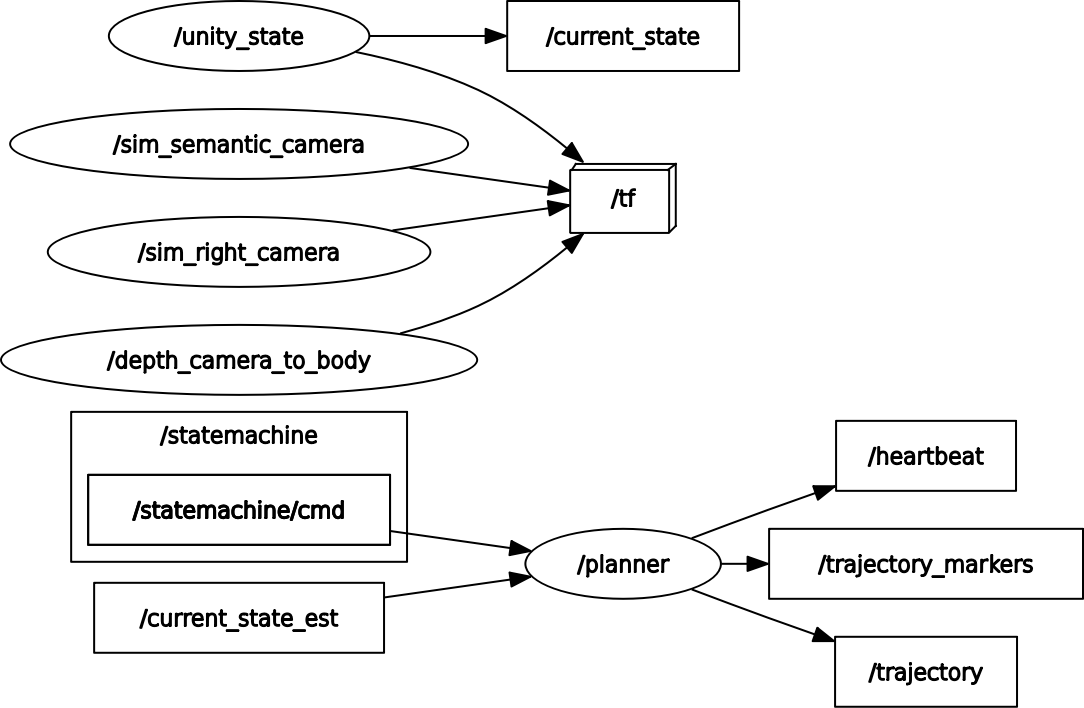
\includegraphics[width=\columnwidth]{figures/rosgraph.png}
  \caption{ROS computation graph during the Subterrain Challenge runtime. }
  \label{fig:rosgraph}
\end{figure}

\subsection{Simulation Interface (Instructor-Provided)}

The simulation infrastructure was provided by the course staff.
The \texttt{simulation} package handles all communication with the Unity simulator.
A TCP client (\texttt{unity\_ros}) connects to Unity, reads binary packets carrying sensor data (RGB, depth, IMU, ground-truth state), and publishes them as standard ROS\,2 messages.
A UDP sender (\texttt{w\_to\_unity}) streams rotor speed commands back at 1\,kHz.
A \texttt{state\_estimate\_corruptor} node injects Gaussian noise and random-walk drift into the ground-truth pose, publishing corrupted odometry on \texttt{/current\_state\_est} to simulate realistic sensor imperfections.
The parsers also handle the left-handed (Unity) to right-handed (ROS) coordinate conversion.

The \texttt{controller\_pkg}, also instructor-provided, implements an SE(3) geometric tracking controller\,\cite{Lee2010} as a precompiled library.
It subscribes to desired trajectory commands and the estimated state, and outputs \texttt{mav\_msgs/Actuators} messages containing the four rotor angular velocities.
The MAV message definitions (\texttt{mav\_msgs}, \texttt{mav\_planning\_msgs}) were ported from the ETH-ASL \texttt{mav\_comm} repository\,\cite{ETHmavcomm}.

\subsection{Perception}

The perception pipeline consists of two cascaded nodes.

\paragraph{Depth to point cloud.}
The \texttt{depth\_to\_pointcloud} node subscribes to the depth camera image (\texttt{16UC1}, millimeters) and the corresponding \texttt{CameraInfo}.
For each pixel it applies the standard pinhole back-projection:
\begin{equation}
  x = \frac{(u - c_x)\,z}{f_x}, \quad
  y = \frac{(v - c_y)\,z}{f_y}
\end{equation}
where $(c_x, c_y)$ is the principal point and $(f_x, f_y)$ the focal lengths.
A configurable downsample factor and a maximum-depth threshold reduce the output size.

\paragraph{Point cloud to OctoMap.}
The \texttt{pointcloud\_to\_octomap} node receives the point cloud, transforms each point from the camera frame to the world frame via TF2, and inserts them into an OctoMap octree\,\cite{Hornung2013}.
We use a resolution of 0.15\,m, with hit probability 0.65, miss probability 0.2, and clamping thresholds of 0.12 and 0.97.
The resulting occupancy grid is published as \texttt{octomap\_msgs/Octomap} and additionally as a colour-coded \texttt{MarkerArray} for visualization in RViz2.

\subsection{Lantern Detection}

The detection node synchronizes the semantic camera image with the depth image using an approximate-time message filter.
It converts the semantic image to grayscale, applies a threshold (intensity~$>10$) to obtain a binary mask, and back-projects the masked pixels to 3D using the same pinhole model.
After transforming to the world frame, the resulting 3D position is compared against a running list of known lanterns.
If a new detection falls within 1.5\,m of an existing entry, the position is updated as a weighted average:
\begin{equation}
  \mathbf{p}_{\text{new}} = \frac{n\,\mathbf{p}_{\text{old}} + \mathbf{p}_{\text{det}}}{n + 1}
\end{equation}
Otherwise, a new lantern is registered.
Detected lanterns are published as both a \texttt{PoseArray} and a yellow \texttt{MarkerArray} for debugging.

\subsection{Path Planning}

Our path planner implements the A* algorithm on a 3D voxel grid\,\cite{Hart1968}.
When a new OctoMap message arrives, the node iterates over all occupied leaf nodes and inflates them by a configurable safety margin (0.5\,m in every direction) to account for the drone's body size.
Occupied voxels are stored in a hash set keyed by a 64-bit integer that encodes three 21-bit signed coordinates, giving $O(1)$ collision checks.

The A* search uses a 26-connected neighbourhood (including diagonals) with a Euclidean heuristic.
We cap the number of expanded nodes at 100\,000 to keep planning times bounded.
After the search, the resulting path is decimated by keeping every third waypoint, which avoids feeding an unnecessarily dense sequence to the trajectory planner.
If no map data is available yet or A* fails to find a path, the planner falls back to a simple 20-point straight-line interpolation toward the goal.


\subsection{Trajectory Planning}

The trajectory planner converts the waypoint path into a time-parameterized \texttt{MultiDOFJointTrajectory} using a trapezoidal velocity profile.
Given a desired cruise speed $v_{\max}$ and maximum acceleration $a_{\max}$, it first computes the acceleration distance:
\begin{equation}
  d_{\text{accel}} = \frac{v_{\max}^2}{2\,a_{\max}}
\end{equation}
If the total path length is too short to reach cruise speed, the acceleration distance is halved.
Each waypoint is then assigned a speed depending on its phase:
\begin{itemize}
  \item \textbf{Acceleration:} $v = \max\!\bigl(\sqrt{2\,a_{\max}\,d},\;0.1\bigr)$
  \item \textbf{Cruise:} $v = v_{\max}$
  \item \textbf{Deceleration:} $v = \max\!\bigl(\sqrt{2\,a_{\max}\,d_{\text{rem}}},\;0.1\bigr)$
\end{itemize}
The velocity vector is aligned with the direction to the next waypoint.
Inter-waypoint time intervals are computed as $\Delta t = d_{\text{seg}} / v_{\text{avg}}$, clipped to a minimum of 0.05\,s.
The last point receives zero velocity so the drone comes to a full stop at the goal.
We use $v_{\max} = 2.0$\,m/s and $a_{\max} = 1.5$\,m/s$^2$ for a stable flight profile.





\subsection{State Machine}

The mission state machine manages the high-level flight sequence.
It cycles through the following states:
\begin{enumerate}
  \item \textbf{INIT} -- wait for the first valid odometry and record the home position.
  \item \textbf{TAKEOFF} -- ascend to 10\,m altitude.
  \item \textbf{TO\_CAVE\_ENTRANCE} -- follow a predefined set of waypoints to reach the cave opening.
  \item \textbf{EXPLORE} -- autonomously explore the cave using frontier-based goals from the mapping module; detect lanterns along the way.
  \item \textbf{RETURN\_HOME} -- navigate back to the recorded home position.
  \item \textbf{LAND} -- descend to 0.4\,m and stop.
  \item \textbf{COMPLETE} -- mission finished.
\end{enumerate}
A 200\,ms tick timer drives transitions.
The exploration phase terminates either when all four lanterns are found or after a 7-minute timeout.
In the exploration state, the node subscribes to frontier goals published by the mapping module and forwards them as \texttt{PoseStamped} goals to the path planner.
An arrival tolerance of 5\,m triggers the transition to the next waypoint or state.

\subsection{Mapping}

The mapping package was designed to maintain a persistent voxel-grid representation alongside frontier-based exploration goals\,\cite{Yamauchi1997}.
Mapping responsibilities are split across mapping and mapping\_pkg. In mapping, nodes such as voxel\_grid\_mapper\_node and global\_map\_publisher\_node maintain voxel/global map products and expose map\_related outputs/services. In mapping\_pkg, octomap\_server\_node builds occupancy maps from point cloud input for planning.

\subsection{Custom Messages and Services}

The \texttt{utils} package defines the shared message and service types used across the system:
\begin{itemize}
  \item \texttt{LanternPose} / \texttt{LanternPoseArray}: detected lantern positions with confidence and confirmation fields.
  \item \texttt{GlobalMap}: full voxel-grid map with occupied, free, and frontier data plus metadata (resolution, explored volume, storage path).
  \item \texttt{SaveMap.srv}: persists the current map to disk.
  \item \texttt{SetMissionMode.srv}: allows manual override of the active FSM state.
\end{itemize}


%%%%%%%%%%%%%%%%%%%%%%%%%%%%%%%%%%%%%%%%%%%%%%%%%%%%%%%%%%%%
\section{Design Choices}

\paragraph{ROS\,2 Jazzy on Ubuntu 24.04.}
ROS\,2 Jazzy\,\cite{Macenski2022} was chosen for its long-term support status and availability on Ubuntu 24.04.
All inter-node communication uses standard topics; services are reserved for on-demand operations like saving the map or overriding the mission mode.

\paragraph{Modular package layout.}
Each functional block lives in its own ROS\,2 package with a dedicated launch file, which let us develop and test components independently.
A master launch file in the \texttt{utils} package can bring everything up at once.

\paragraph{OctoMap for 3D occupancy.}
We used the OctoMap library\,\cite{Hornung2013,OctomapROS} rather than a flat voxel array because its octree compression reduces memory usage for large cave environments while still supporting ray casting and probabilistic updates.

\paragraph{A* path planning.}
We considered RRT and its variants, but A* on a discretised voxel grid offers deterministic, resolution-complete paths with straightforward obstacle inflation.
With a 0.15\,m resolution and a 100\,k node expansion budget, planning finishes well within real-time constraints.

\paragraph{Trapezoidal velocity profile.}
A polynomial trajectory (e.g.\ minimum-snap) would produce smoother motion, but the trapezoidal profile is simpler to implement, easier to tune, and gives predictable acceleration/deceleration phases that are sufficient for cave navigation at 2\,m/s cruise speed.

%%%%%%%%%%%%%%%%%%%%%%%%%%%%%%%%%%%%%%%%%%%%%%%%%%%%%%%%%%%%
\section{Limitations and Known Issues}

Several modules are architecturally designed but not yet fully implemented.
The \texttt{mapping} node (persistent voxel grid and frontier goals), the \texttt{state\_machine} (mission FSM sequencing), and the \texttt{quadrotor\_controller} (100\,Hz trajectory sampler) all have complete header definitions and parameter files, but their callback bodies remain as TODO placeholders.
As a result, the system does not yet autonomously sequence the full mission (take-off, cave entry, exploration, return, landing); navigation currently requires manual goal publication.
The \texttt{perception\_pipeline} package was planned as an extended alternative to the \texttt{perception} and \texttt{detection} nodes---with semantic mask filtering and \texttt{LanternPoseArray} output---but was not completed.

Another limitation is that the OctoMap is rebuilt from scratch every frame rather than accumulated over time, which means the path planner only sees obstacles currently in the field of view.
A persistent map would require the mapping module, which is not yet functional.

%%%%%%%%%%%%%%%%%%%%%%%%%%%%%%%%%%%%%%%%%%%%%%%%%%%%%%%%%%%%
\section{Results}

\begin{figure}
  \centering
  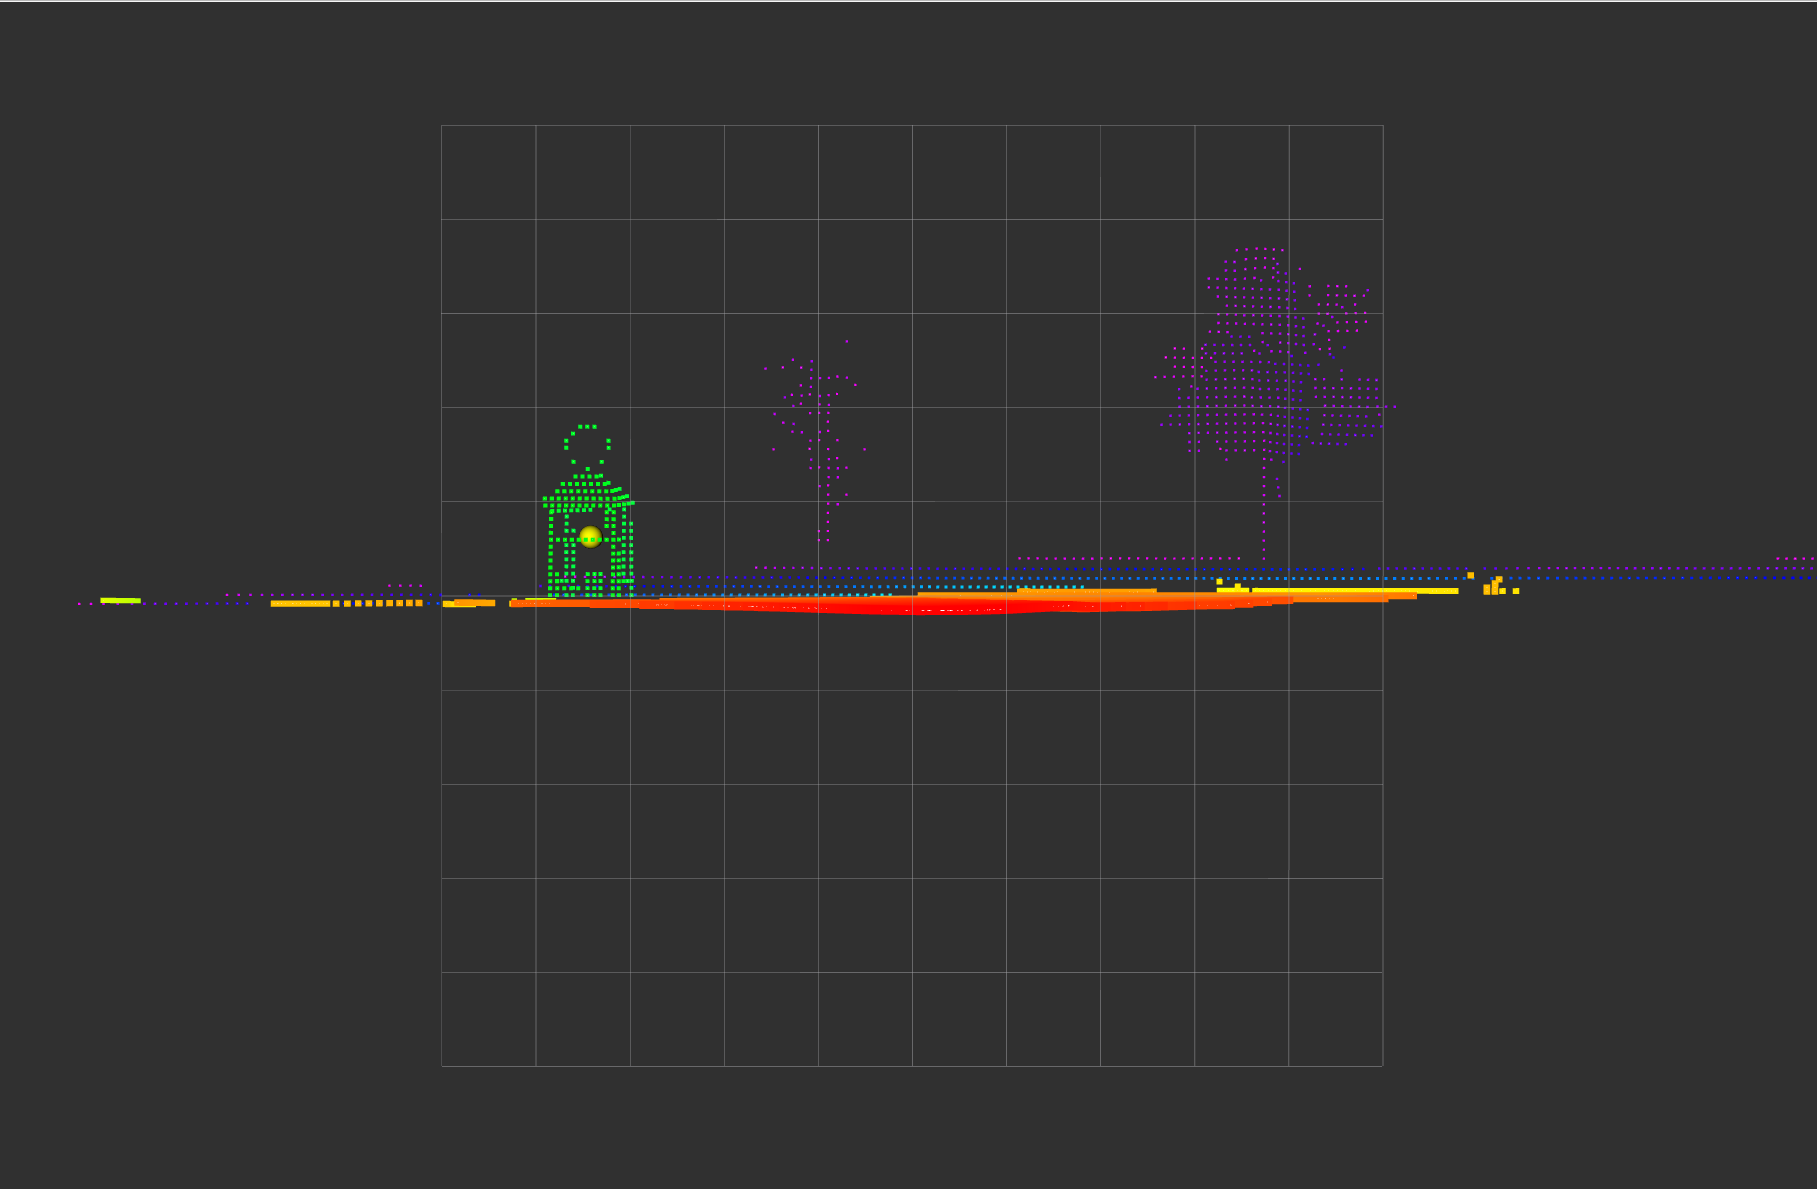
\includegraphics[width=\columnwidth]{figures/rviz2.png}
  \caption{Visualization in RViz2 showing the OctoMap occupancy grid (coloured by height), the drone's estimated pose (TF frame), and detected lanterns (yellow spheres).}
  \label{fig:rviz}
\end{figure}

With the perception pipeline running, the system produces dense OctoMap updates and successfully detects lanterns when they enter the semantic camera's field of view.
The path planner generates collision-free paths in real time, and the trajectory planner provides smooth velocity profiles that the SE(3) controller tracks reliably.
Figure~\ref{fig:rviz} shows a representative RViz2 snapshot during a test run.

%%%%%%%%%%%%%%%%%%%%%%%%%%%%%%%%%%%%%%%%%%%%%%%%%%%%%%%%%%%%
\section{Code Attribution and Contributions}

\subsection{External Code}

The following components were provided by the course or taken from external sources:
\begin{itemize}
  \item \texttt{simulation} package -- complete Unity--ROS\,2 bridge (TCP/UDP communication, sensor parsers, state corruptor, TF publishers, launch files). Provided by the course staff.
  \item \texttt{controller\_pkg} -- SE(3) geometric controller with precompiled \texttt{libcontroller\_lib.so}. Provided by the course staff\,\cite{Lee2010}.
  \item \texttt{mav\_msgs} and \texttt{mav\_planning\_msgs} -- MAV message definitions ported from ETH-ASL \texttt{mav\_comm}\,\cite{ETHmavcomm}. Provided with the course material.
  \item OctoMap library\,\cite{Hornung2013} -- used via system packages.
  \item \texttt{libsocket} -- third-party TCP/UDP socket library, fetched at build time by the simulation package.
\end{itemize}

\subsection{Contribution Matrix}

Table~\ref{tab:contributions} summarises who worked on which packages.

\begin{table}[h]
\centering
\caption{Package contributions per team member.}
\label{tab:contributions}
\small
\begin{tabularx}{\columnwidth}{lX}
\toprule
\textbf{Member} & \textbf{Packages / Responsibilities} \\
\midrule
Iliasu Salaudeen & \texttt{state\_machine}, \texttt{controller\_pkg} integration: mission FSM architecture, controller launch configuration \\
Jiacheng Li & \texttt{perception}, \texttt{detection}: depth-to-pointcloud, OctoMap integration, lantern detector with semantic+depth fusion \\
Nihat Ak{\i}n & \texttt{path\_planner}, \texttt{trajectory\_planner}: A* search on inflated voxel grid, trapezoidal velocity profiling, waypoint decimation \\
Yujia Wang & \texttt{mapping}, \texttt{utils}, \texttt{perception\_pipeline}: voxel grid mapper architecture, custom messages/services, master launch file, system integration \\
Ziming Liu & \texttt{mapping}, \texttt{quadrotor\_controller}: simulation integration, trajectory sampler architecture, system-wide testing \\
\bottomrule
\end{tabularx}
\end{table}

All members contributed to debugging, testing, and the written report.

%%%%%%%%%%%%%%%%%%%%%%%%%%%%%%%%%%%%%%%%%%%%%%%%%%%%%%%%%%%%
\section*{Acknowledgements}
We thank the Autonomous Systems teaching team at TUM for providing the simulation environment, base code, and support throughout the project.

\printbibliography

\end{document}